% !TeX program = xelatex
% =====================================================================
%  风电场高保真物理仿真平台 —— 框架 / 愿景汇报 Slides
%  面向教授的框架类汇报：重意义与定位，专业术语用英文并附解释，
%  强化学习与疲劳载荷单独讲透，物理严谨性用可验证的例子撑。
%
%  编译：xelatex vision_slides.tex（跑两次以生成目录/页码）
%  依赖：ctexbeamer（TeXLive / CTeX 自带），需 XeLaTeX
%  Overleaf：Menu -> Compiler 选 XeLaTeX，figs/ 目录随 .tex 一起上传。
%          ctexbeamer 在 Overleaf 走 Fandol 字体，不要加 fontset=windows。
% =====================================================================
\documentclass[aspectratio=169,10pt,UTF8]{ctexbeamer}

\usetheme{Madrid}
\usecolortheme{whale}
\setbeamertemplate{navigation symbols}{}
\setbeamertemplate{caption}[numbered]
\setbeamercovered{transparent}
\setbeamerfont{frametitle}{size=\normalsize}

\usepackage{amsmath,amssymb,amsfonts,mathtools}
\usepackage{bm}
\usepackage{booktabs}
\usepackage{array}
\usepackage{tikz}
\usetikzlibrary{arrows.meta,positioning,shapes.geometric,calc}
\usepackage{graphicx}

% ---- 颜色 ----
\definecolor{myblue}{RGB}{20,80,140}
\definecolor{myred}{RGB}{170,40,40}
\definecolor{mygreen}{RGB}{30,110,70}
\definecolor{myorange}{RGB}{200,110,20}
\setbeamercolor{block title}{bg=myblue!15,fg=myblue!80!black}

% ---- 小助手 ----
\newcommand{\hl}[1]{{\color{myblue}\bfseries #1}}
\newcommand{\hlr}[1]{{\color{myred}\bfseries #1}}
\newcommand{\hlg}[1]{{\color{mygreen}\bfseries #1}}
% 术语：英文 + 中文解释，首次出现用
\newcommand{\term}[2]{\textbf{#1}\,（#2）}

\title[风电场高保真物理仿真平台]{面向风电场的高保真物理仿真平台}
\subtitle{以物理规律为约束的工业应用预演环境}
\author{课题组汇报}
\date{\today}

\begin{document}

% =====================================================================
\begin{frame}[plain]
  \titlepage
  \begin{center}
    \small\itshape
    High-fidelity physics simulation \,$+$\, reinforcement-learning control
    \,$+$\, industrial pre-deployment
  \end{center}
\end{frame}

% =====================================================================
\begin{frame}{提纲与定位}
  \begin{columns}[T]
    \begin{column}{0.6\textwidth}
      \textbf{一句话定位}
      \begin{itemize}\small
        \item 面向风电场的\hl{高保真物理仿真平台}：让控制策略与工业应用在
              \textbf{上机之前}先在虚拟风场中试运行；
        \item 类比（仅定位、不展开）：机器人领域用物理仿真把策略先练好再上真机
              （\term{sim-to-real}{仿真到现实}）——风电场同样需要这样一个平台。
      \end{itemize}
      \vspace{0.4em}
      \textbf{本汇报的逻辑主线}
      \begin{enumerate}\small
        \item 时代背景与迫切性（policy / market / O\&M）
        \item 平台意义与目标
        \item 物理严谨性及其可验证性
        \item 强化学习控制：为何必要
        \item 疲劳载荷估计：如何可信
        \item 当前实现与下一步
      \end{enumerate}
    \end{column}
    \begin{column}{0.4\textwidth}
      \begin{block}{关键立场}
        \small 平台的价值 $=$ 预演结论\hlr{可外推到现场}；
        其前提 $=$ 仿真\hl{严格遵守物理规律}。
        本汇报重点论证这个前提\textbf{已经成立}。
      \end{block}
    \end{column}
  \end{columns}
\end{frame}

% =====================================================================
\begin{frame}{术语表（Glossary）}
  \small
  \begin{columns}[T]
    \begin{column}{0.5\textwidth}
      \begin{itemize}\small
        \item \textbf{aeroelastic} —— 气动弹性：气动力与结构弹性变形耦合求解
        \item \textbf{wake} —— 尾流：机组下游被吸走能量、湍流增强的风区
        \item \textbf{wake steering} —— 尾流偏转：主动偏航把尾流推离下游机组
        \item \textbf{DWM} —— dynamic wake meandering，动态尾流蜿蜒
        \item \textbf{TSR} —— tip-speed ratio，叶尖速比（叶尖线速度/来流风速）
        \item \textbf{yaw / pitch / torque} —— 偏航 / 变桨 / 发电机转矩
      \end{itemize}
    \end{column}
    \begin{column}{0.5\textwidth}
      \begin{itemize}\small
        \item \textbf{DEL} —— damage equivalent load，等值疲劳载荷
        \item \textbf{rainflow counting} —— 雨流计数（提取应力循环，ASTM E1049）
        \item \textbf{S-N curve} —— 应力幅–寿命曲线（材料疲劳特性）
        \item \textbf{Miner's rule} —— 线性累积损伤准则
        \item \textbf{O\&M} —— operation \& maintenance，运行与维护
        \item \textbf{MAPPO / CTDE} —— 多智能体 PPO / 集中训练分散执行
      \end{itemize}
    \end{column}
  \end{columns}
\end{frame}

% =====================================================================
\section{时代背景与迫切性}

\begin{frame}{迫切性（一）：政策与市场的双重驱动}
  \begin{columns}[T]
    \begin{column}{0.5\textwidth}
      \textbf{政策侧}
      \begin{itemize}\small
        \item “双碳”目标下，风电是主力可再生能源，\hl{新增装机持续高位增长}；
        \item 存量机组规模不断扩大，\term{O\&M}{运维}成本占全生命周期成本
              相当比重，降本压力直接落在运维效率。
      \end{itemize}
      \vspace{0.3em}
      \textbf{市场侧}
      \begin{itemize}\small
        \item 电力市场化推进，风场需\hl{按市场需求 $+$ 实时风况动态调度}；
        \item 从“并网即消纳”转向\textbf{主动参与市场}，对控制与预测的要求上升。
      \end{itemize}
    \end{column}
    \begin{column}{0.5\textwidth}
      \begin{block}{一句话}
        \small 装机在\hl{扩张}、运维成本在\hl{累积}、市场在\hl{放开}——
        三条曲线共同抬高了对“更聪明的控制”与“更低成本的验证手段”的需求。
      \end{block}
      \vspace{0.6em}
      \begin{center}\scriptsize\color{gray}
        注：具体装机量 / 运维成本占比数字，汇报时按最新行业报告填入。
      \end{center}
    \end{column}
  \end{columns}
\end{frame}

\begin{frame}{迫切性（二）：风电智能化对高保真仿真的依赖}
  \begin{itemize}\small
    \item \hl{智能运维（intelligent O\&M）}正在发生：无人机巡检、机舱智能相机监测
          叶片、\term{vibration}{振动} 与 \term{acoustic}{声发射}健康监测；
    \item \hl{风机“智驾”}：从固定控制律（fixed control law）走向\textbf{数据驱动的
          智能协同控制}；
    \item 这些智能应用的开发、验证、调优\hlr{高度依赖高保真物理仿真}——
          正如自动驾驶（autonomous driving）离不开仿真：真实路测昂贵且危险，
          绝大部分里程在仿真里跑完。
  \end{itemize}
  \vfill
  \begin{block}{类比自动驾驶}
    \small 自动驾驶：\textbf{仿真里跑百万公里}，把长尾场景与危险工况前移到虚拟世界。\\
    风电场：\textbf{仿真里跑百万控制步}，把昂贵、缓慢、危险的现场试验前移到虚拟风场。
  \end{block}
\end{frame}

\begin{frame}{迫切性（三）：没有仿真平台时的现场约束}
  \begin{columns}[T]
    \begin{column}{0.5\textwidth}
      \textbf{一切依赖“人上现场”}
      \begin{itemize}\small
        \item 传感器安装、相机挂机方案，靠技术人员\hlr{出差、登机、人工上机}
              反复试 —— 成本高、周期长、有高空作业风险；
        \item 方案不合适（相机拍不到目标、角度不对）需\textbf{再上机一次}；
        \item 控制策略现场试验 $=$ \hlr{真实停机与发电损失}，且不可回退。
      \end{itemize}
    \end{column}
    \begin{column}{0.5\textwidth}
      \textbf{部分数据现场根本采不到}
      \begin{itemize}\small
        \item \hlr{极端/恶劣工况}（台风、结冰、强湍流）可遇不可求，
              等真发生往往已是事故；
        \item 但这些工况\hl{可按物理规律模拟}——游戏引擎尚能造风造浪，
              严格的 \term{aeroelastic}{气动弹性}仿真更能给出可信响应；
        \item \hlr{长期稳定性}（疲劳累积，历时数月至数年）现场无法压缩验证，
              仿真可\textbf{加速推演}。
      \end{itemize}
    \end{column}
  \end{columns}
  \vfill
  \begin{center}
    \hl{结论：风电场比以往更需要一个“可信的预演场”——“可信” $=$ 严格遵守物理规律。}
  \end{center}
\end{frame}

% =====================================================================
\section{平台意义与目标}

\begin{frame}{平台意义：把现场做不到的变为可做}
  \begin{columns}[T]
    \begin{column}{0.5\textwidth}
      \textbf{仿真所独有的能力}
      \begin{itemize}\small
        \item \hlg{任意重复、并行、清零}：同一方案换参数跑上百遍，零边际成本；
        \item 把“数十秒才显现的\term{wake}{尾流}–载荷–控制耦合”压缩到可反复观测；
        \item 极端工况\textbf{按需生成}，不必等其真实发生；
        \item 长期疲劳\textbf{加速推演}，无需数月现场跟踪。
      \end{itemize}
    \end{column}
    \begin{column}{0.5\textwidth}
      \textbf{把上机风险前移到虚拟场}
      \begin{itemize}\small
        \item 控制策略可训练\textbf{百万量级}而不损伤任何设备；
        \item 传感器/相机安装方案\textbf{先预演、再出差上机}；
        \item 新控制律的安全边界\textbf{先在仿真里探清}；
        \item 失败在仿真里随时回退，现场失败不可回退。
      \end{itemize}
    \end{column}
  \end{columns}
  \vfill
  \begin{center}\small
    \hl{前提：仿真必须“可信”——即严格遵守物理规律，否则预演结论不能外推到现场。}
  \end{center}
\end{frame}

\begin{frame}{平台目标：物理 $+$ 感知 $+$ 控制 $+$ 预演}
  \begin{center}
  \begin{tikzpicture}[node distance=0.7cm and 1.2cm,
      box/.style={draw,rounded corners,fill=myblue!8,text width=3.1cm,
        align=center,minimum height=1.0cm,font=\small},
      arr/.style={-{Latex[length=2mm]},thick,myblue}]
    \node[box] (sim) {\textbf{物理保真仿真}\\aeroelastic $+$ wake};
    \node[box,right=of sim] (sensor) {\textbf{多模态传感}\\camera/lidar/vibration/acoustic};
    \node[box,right=of sensor] (ctrl) {\textbf{智能控制}\\RL $+$ safety constraint};
    \node[box,below=of sensor,fill=mygreen!12] (ind)
      {\textbf{工业应用预演}\\上机前先试运行};
    \draw[arr] (sim) -- (sensor);
    \draw[arr] (sensor) -- (ctrl);
    \draw[arr] (sim) -- (ind);
    \draw[arr] (sensor) -- (ind);
    \draw[arr] (ctrl) -- (ind);
  \end{tikzpicture}
  \end{center}
  \vfill
  \begin{itemize}\small
    \item 一个平台，把\hl{物理、感知、控制}接在同一套虚拟风场里；
    \item 风场专业人员可\hlg{创建风场、导入数据通道、预演工业方案}，并在 3D 中观测全程；
    \item 长远目标：使\textbf{“先在仿真里预演”}成为风电场工程的默认工作方式。
  \end{itemize}
\end{frame}

% =====================================================================
\section{物理严谨性}

\begin{frame}{物理严谨性（一）：数据的三级保真度}
  \begin{center}
    \hlr{预演结论能否外推，取决于物理准不准。}\ 平台把数据来源\textbf{显式分级}：
  \end{center}
  \vspace{0.3em}
  \begin{block}{三级保真度（fidelity），混用会使结论失效}
    \begin{itemize}\small
      \item \hlg{DIRECT（直读）}：仿真器直接算出的量——功率、叶根弯矩、桨距、
            转矩、偏航。\textbf{可进入控制与安全判据}；
      \item \hl{DERIVED（导出）}：由直读量按明确物理公式推得，例如转子转速由
            $\omega_{\text{gen}} = P/(\eta\,T)$ 反解、再除齿轮箱速比；
      \item \textbf{SYNTH（合成）}：为观感造的模型（如尾流包络动画）——
            \hlr{只进画面，绝不进入奖励或安全约束}。
    \end{itemize}
  \end{block}
  \begin{center}\small
    每一路数据都标注\textbf{来源与保真度}——汇报任一结论时，能说清它是“算出来的”
    还是“画出来的”。
  \end{center}
\end{frame}

\begin{frame}{物理严谨性（二）：底层是气动弹性仿真，非解析近似}
  \begin{columns}[T]
    \begin{column}{0.56\textwidth}
      \begin{itemize}\small
        \item 底层求解器为 \hl{FAST.Farm}（美国 NREL）：\term{aeroelastic}{气动弹性}
              内核 $+$ \term{DWM}{动态尾流蜿蜒}，\textbf{真实时间推进}、有惯性与历史；
        \item 机组为 NREL 5\,MW 参考机型\textbf{真实几何}：翼型、弦长、扭角、锥角
              （precone）、轴倾（tilt）、悬伸（overhang）均取自 OpenFAST 模板；
        \item 叶片按叶根弯矩\textbf{柔性变形}并做\textbf{扫塔间隙（tower clearance）}
              计算——叶尖离塔多近是\hl{算出来}的，不是画的。
      \end{itemize}
      \vspace{0.3em}
      \begin{block}{对照：稳态解析模型的局限}
        \small 稳态解析尾流模型（如 FLORIS）快、适合大规模训练，但没有时间维；
        高保真验证必须回到 aeroelastic 仿真。二者\textbf{共用同一套接口}，可作
        受控对照（下页）。
      \end{block}
    \end{column}
    \begin{column}{0.44\textwidth}
      \centering
      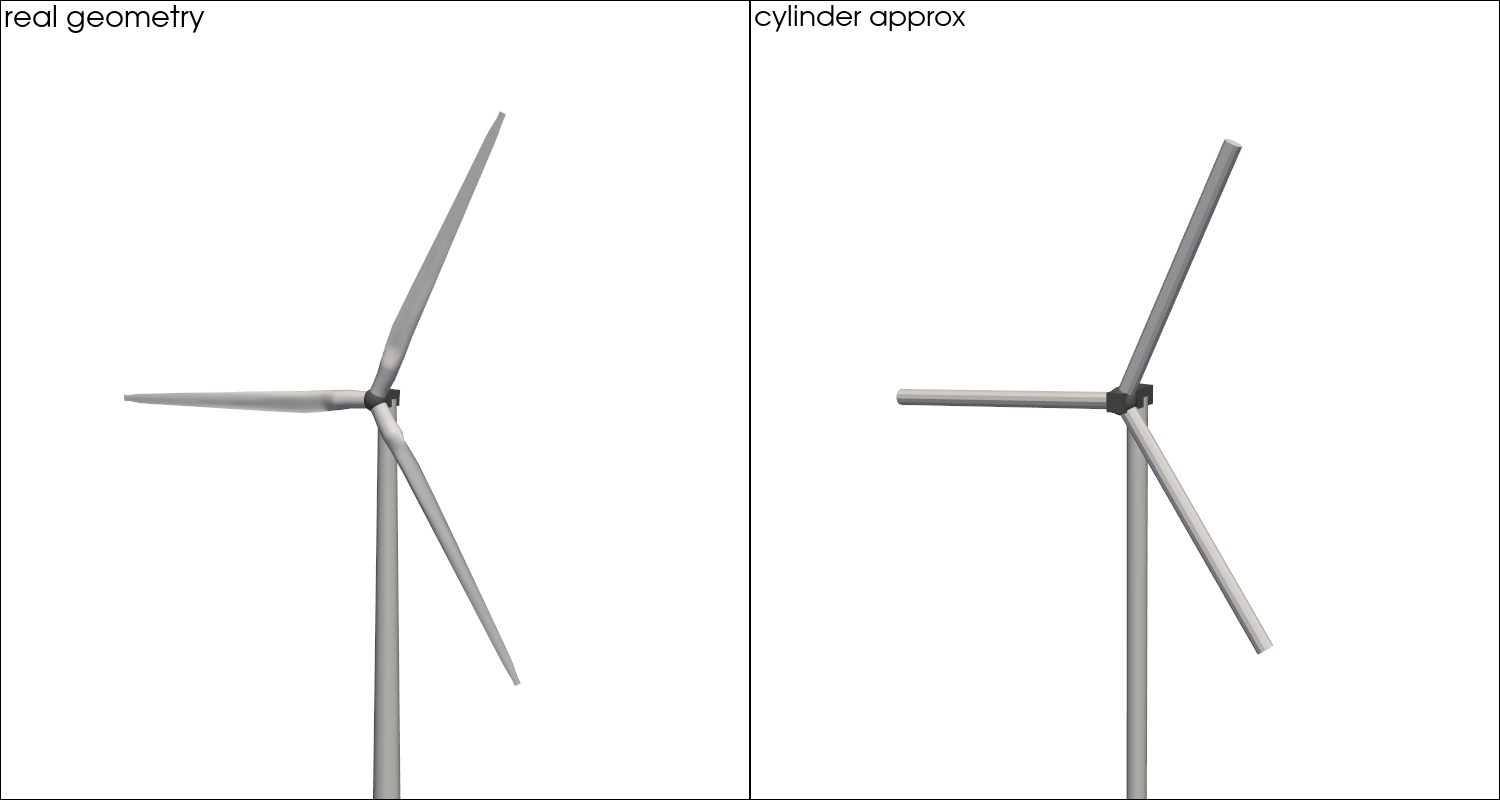
\includegraphics[width=\linewidth]{figs/fig_geom_real.png}\\
      {\scriptsize NREL 5\,MW 真实几何（叶片放样、轴倾、悬伸）}
    \end{column}
  \end{columns}
\end{frame}

\begin{frame}{物理严谨性（三）：一个可验证的对照结论}
  \begin{columns}[T]
    \begin{column}{0.5\textwidth}
      \begin{itemize}\small
        \item 同一来流下，稳态解析模型比气动弹性仿真\hlr{低估下游功率 13--18\%}，
              且差异\textbf{全部集中在下游机组}；
        \item 物理解释：气动弹性里有\term{wake}{尾流}蜿蜒与湍流掺混带来的
              \textbf{动量恢复}，稳态模型无法体现；
        \item \term{wake}{尾流}对下游的完整影响\hl{滞后约 46 个控制步}才建立——
              这类时延，只有真实时间推进的物理才拿得到。
      \end{itemize}
      \vspace{0.2em}
      \begin{center}\scriptsize
        这类“可复现、可解释”的差异，正是“物理真的实现了”的\textbf{可验证证据}。
      \end{center}
    \end{column}
    \begin{column}{0.5\textwidth}
      \centering
      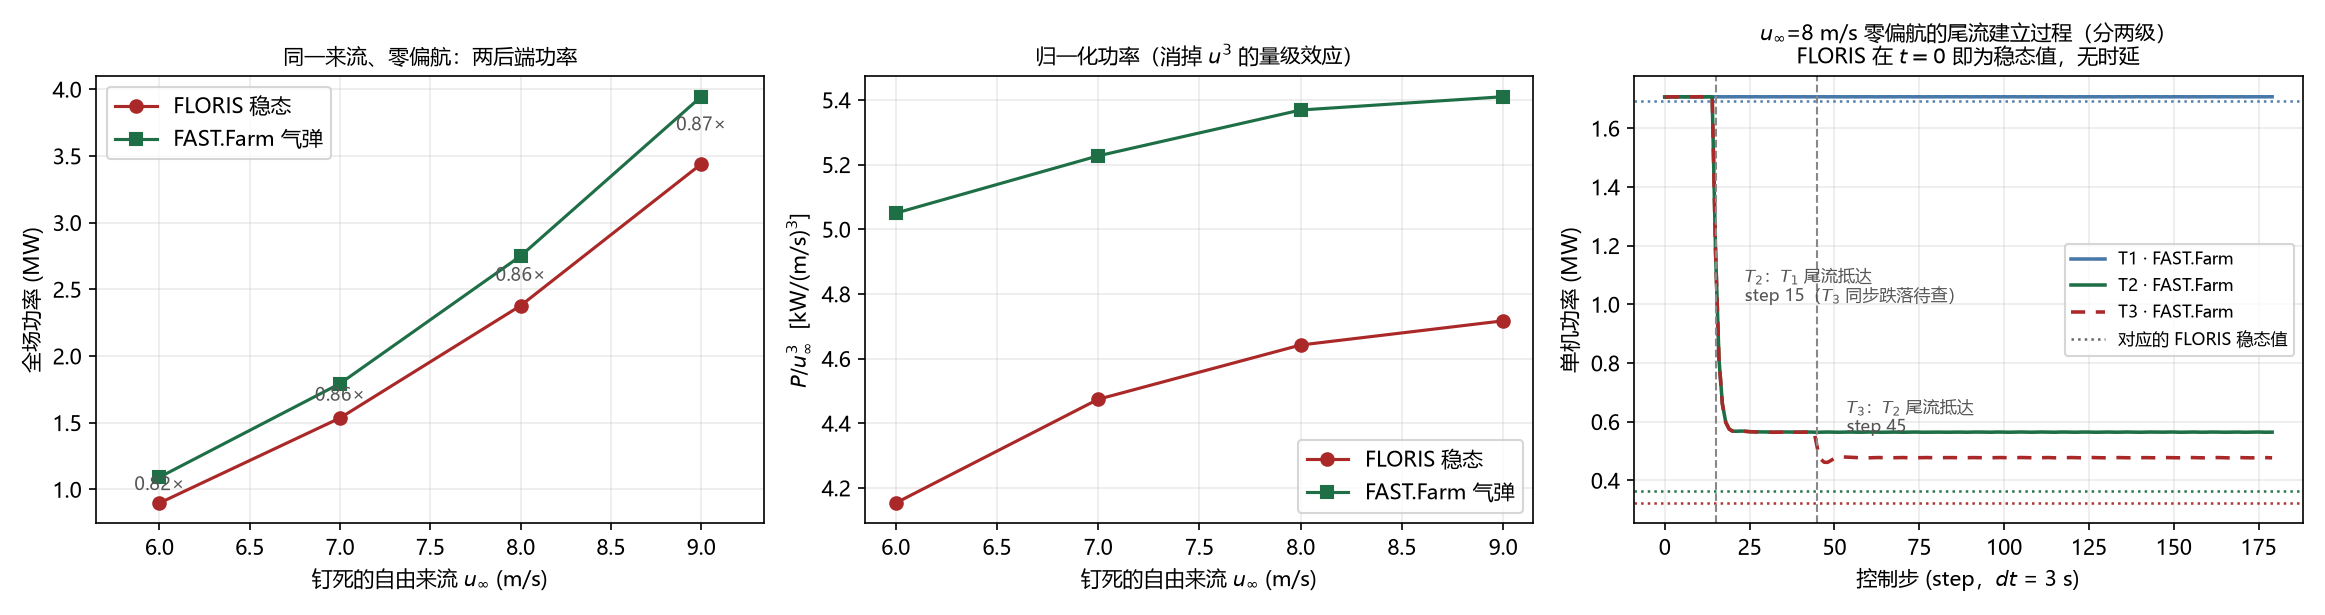
\includegraphics[width=\linewidth]{figs/fig_control_matched.png}\\
      {\scriptsize 钉死来流下的双后端对照（稳态 vs 气动弹性）}
    \end{column}
  \end{columns}
\end{frame}

\begin{frame}{物理严谨性（四）：控制指令须过物理与安全约束层}
  \begin{center}\small
    策略网络输出无量纲实数；它与“可下发指令”之间隔一层\hl{physics \& safety
    constraint layer（物理与安全约束层）}——\textbf{无论策略学成什么样，下发动作都合物理}。
  \end{center}
  \vspace{0.2em}
  \begin{columns}[T]
    \begin{column}{0.6\textwidth}
      \begin{block}{仿真侧会“悄悄改写”不合规动作，平台将其显式建模}
        \begin{itemize}\scriptsize
          \item \textbf{执行机构占空比（actuator duty cycle）}：偏航电机不能持续动，
                超上限则该步指令被\hlr{整步清零}（非限幅）；
          \item \textbf{变桨是下界非指令}：外部 pitch 低于基线控制器时\textbf{无效}；
          \item \textbf{发电机转矩完全顶替基线}：转矩过大将把转子\hlr{刹至失速}
                （\term{TSR}{叶尖速比}$\approx 2$、气动求解关闭、转子停转）。
        \end{itemize}
      \end{block}
      \vspace{-0.2em}
      \begin{center}\scriptsize
        约束层把转矩\textbf{锚定在维持最优 TSR 的曲线上}（既防超速又防失速），
        并\textbf{逐条记录}每次被改写的动作。
      \end{center}
    \end{column}
    \begin{column}{0.4\textwidth}
      \centering
      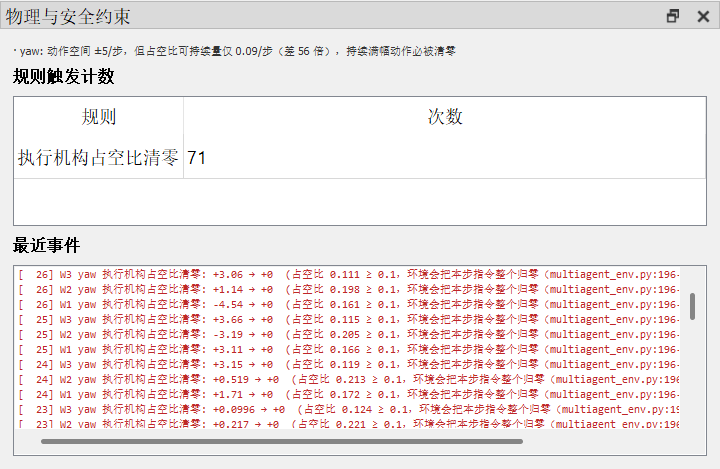
\includegraphics[width=\linewidth]{figs/fig_studio_safety.png}\\
      {\scriptsize 安全约束面板：逐条显示被改写的动作}
    \end{column}
  \end{columns}
\end{frame}

\begin{frame}{数据遵守物理}
  \begin{center}\small
    面向严谨受众，我们不止说“像”，而是给出\hl{可核验的证据链}：
  \end{center}
  \begin{columns}[T]
    \begin{column}{0.5\textwidth}
      \begin{block}{证据}
        \begin{itemize}\scriptsize
          \item \hlg{可追溯}：每一路数据标注来源与保真度（DIRECT/DERIVED/SYNTH）；
          \item \hlg{可复现}：来流可钉死，双后端受控对照，结论有对照支撑；
          \item \hlg{逐位一致}：约束层对“环境将如何改写动作”的预测，
                与仿真实际执行\textbf{逐位吻合}；
          \item \hlg{可证伪}：不可信的数字被撤回并记录原因。
        \end{itemize}
      \end{block}
    \end{column}
    \begin{column}{0.5\textwidth}
      \begin{block}{方法学}
        \begin{itemize}\scriptsize
          \item 底层是社区验证过的 NREL FAST.Farm，非自研简化模型；
          \item 常数（齿轮箱速比、发电机效率、额定转矩等）均有\textbf{出处}；
          \item 合成量（SYNTH）\textbf{严格隔离}在感知/观感层，不污染物理结论。
        \end{itemize}
      \end{block}
      \begin{center}\scriptsize
        \hl{“可信”不是形容词，是一组可检验的性质。}
      \end{center}
    \end{column}
  \end{columns}
\end{frame}

% =====================================================================
\section{强化学习控制：为何必要}

\begin{frame}{强化学习（一）：协同优化决策}
  \begin{columns}[T]
    \begin{column}{0.56\textwidth}
      \begin{itemize}\small
        \item 目标——\term{wake steering}{尾流偏转}：上游机组主动偏航，把
              \term{wake}{尾流}推离下游，\textbf{牺牲自身出力换全场功率净增}；
        \item 这是一个\hl{序贯决策问题}：动作（偏航/变桨/转矩增量）改变流场，
              流场又反过来影响下一步的最优动作；
        \item 耦合出现在\textbf{全场奖励}里——单机看不到全局，必须协同。
      \end{itemize}
      \vspace{0.3em}
      \begin{block}{难点}
        \small 跨机组耦合 $+$ 数十秒时延 $+$ 湍流非平稳 $+$ 高维风况$\times$布局空间
        —— 没有现成公式给出“此刻各机组的最优偏航”。
      \end{block}
    \end{column}
    \begin{column}{0.44\textwidth}
      \centering
      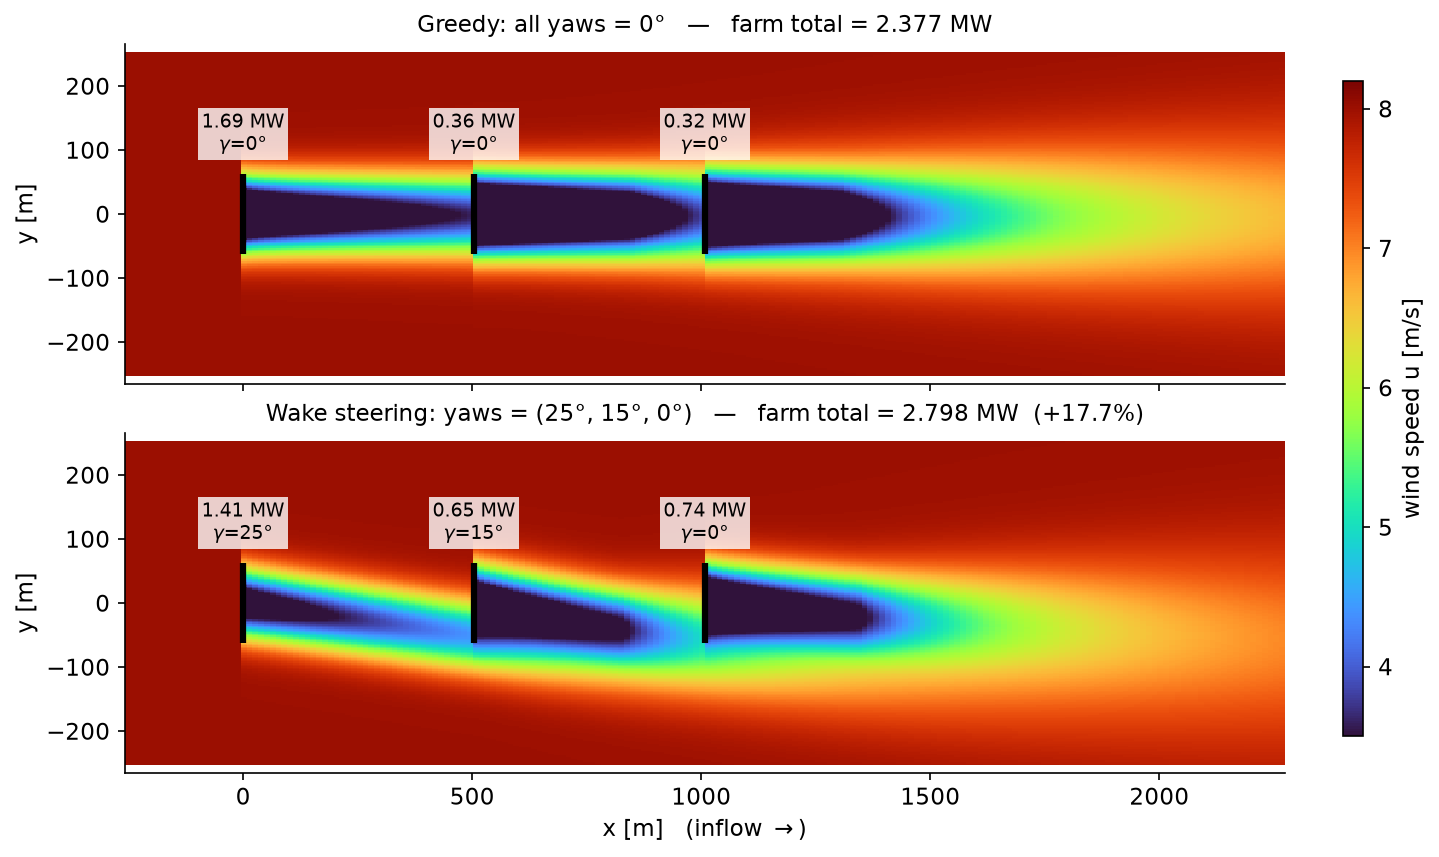
\includegraphics[width=\linewidth]{figs/fig_wake_steering.png}\\
      {\scriptsize 尾流偏转的协同控制}
    \end{column}
  \end{columns}
\end{frame}

\begin{frame}{强化学习（二）：监督学习 / 人类反馈不适用}
  \begin{columns}[T]
    \begin{column}{0.5\textwidth}
      \textbf{监督学习（supervised）不适用}
      \begin{itemize}\small
        \item 监督学习需要\hlr{“正确答案”标签}；而“此刻各机组的最优偏航”
              \textbf{没有标签}——它正是我们要求解的未知量；
        \item 最优解随风速、风向、布局、湍流实时变化，\textbf{无法预先枚举成
              训练集}。
      \end{itemize}
      \vspace{0.2em}
      \textbf{人类反馈 / 示范也不适用}
      \begin{itemize}\small
        \item 人类难以对\textbf{数十秒延迟、跨机组耦合}的后果给出可靠即时评价；
        \item 人工整定只覆盖少数工况，\hlr{泛化不到高维风况空间}。
      \end{itemize}
    \end{column}
    \begin{column}{0.5\textwidth}
      \begin{block}{强化学习恰好匹配这个问题}
        \small
        \begin{itemize}\small
          \item 用\hl{奖励（reward）}而非标签：奖励 $=$ 全场功率（可含载荷惩罚），
                \textbf{可直接测量}；
          \item 用\hl{试错 $+$ 延迟回报}处理时延与信用分配（credit assignment）；
          \item 在\textbf{仿真里}安全试错百万次，正是仿真平台存在的意义。
        \end{itemize}
      \end{block}
      \begin{center}\scriptsize
        一句话：\hl{没有老师给标准答案，只能靠环境的反馈自己学} —— 这就是 RL。
      \end{center}
    \end{column}
  \end{columns}
\end{frame}

\begin{frame}{强化学习（三）：方法有理论依据（MAPPO / CTDE）}
  \begin{columns}[T]
    \begin{column}{0.56\textwidth}
      \begin{itemize}\small
        \item 每台机组是一个\hl{agent}；采用\term{MAPPO}{多智能体近端策略优化}——
              策略梯度类方法（policy gradient），有收敛与稳定性分析支撑；
        \item \term{CTDE}{集中训练、分散执行}：训练时\hl{集中式 critic（评论家）}
              用全局状态评估回报，执行时每个 \hl{actor（策略）}只看\textbf{本机
              局部观测}——落地时不需要全局通信；
        \item 全场共享奖励 $\Rightarrow$ 一个标量优势广播给各机组做策略更新；
        \item \hlr{关键}：actor 输出经\textbf{物理与安全约束层}核验后才下发——
              稳定性由约束层保证，\textbf{与训练好坏无关}。
      \end{itemize}
    \end{column}
    \begin{column}{0.44\textwidth}
      \centering
      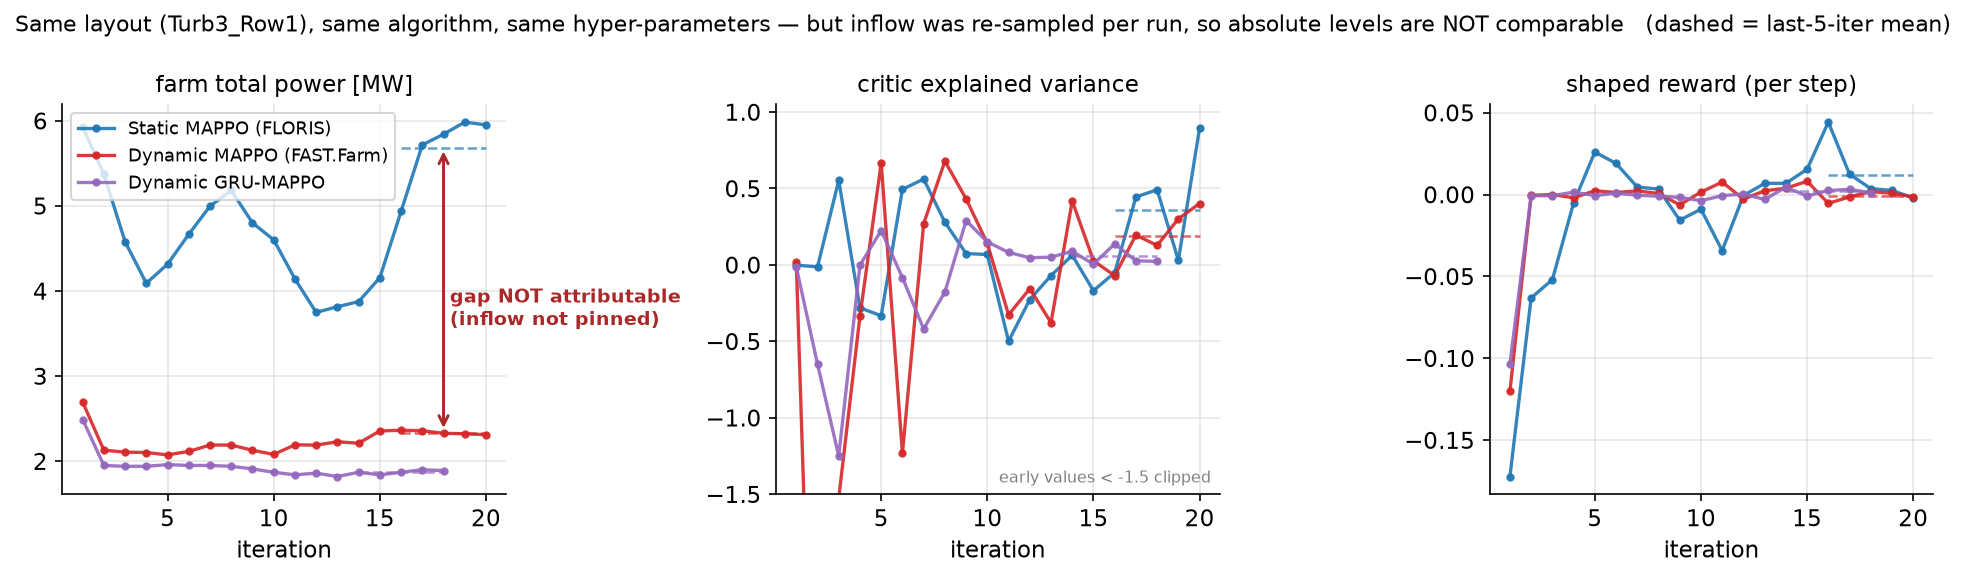
\includegraphics[width=\linewidth]{figs/fig_training.png}\\
      {\scriptsize 后台训练：功率 / 奖励曲线实时可见}
    \end{column}
  \end{columns}
\end{frame}

\begin{frame}{强化学习（四）：重要性}
  \begin{itemize}\small
    \item \hl{学出人类难以手工整定的协同策略}：在跨机组耦合与时延下，找到牺牲局部、
          换取全场净增的偏航配置；
    \item \hl{可迁移、可泛化}：目标是得到在不同风况、不同布局下都成立的策略，
          而非一组固定角度；
    \item \hl{可与安全/寿命目标统一}：奖励可纳入\textbf{疲劳载荷惩罚}，把“多发电”
          与“少损伤”放进同一优化目标（见后）；
    \item \hl{仿真平台是前提}：百万次安全试错只能在物理保真的虚拟风场里完成——
          这把“RL 控制”与“物理仿真平台”\textbf{绑成一件事}。
  \end{itemize}
  \vfill
  \begin{center}\small
    RL 不是为用而用：它是\hlr{“无标签、强耦合、长时延”}这类问题的\textbf{对口方法}。
  \end{center}
\end{frame}

% =====================================================================
\section{多模态感知与疲劳载荷}

\begin{frame}{多模态感知：传感器即数据通道}
  \begin{columns}[T]
    \begin{column}{0.5\textwidth}
      \begin{itemize}\small
        \item \hl{camera（相机）}：机舱相机监测叶片，验证挂机方案（见后页）；
        \item \hl{lidar（激光雷达）}：机舱前视测风，前馈来流（feedforward）；
        \item \hl{vibration（振动）}：由叶根弯矩序列取 1P/3P 谱线与 RMS；
        \item \hl{acoustic（声发射）}：叶片裂纹/结冰的健康指标。
      \end{itemize}
    \end{column}
    \begin{column}{0.5\textwidth}
      \begin{block}{设计原则}
        \small 每个传感器 $=$ 安装位姿 $+$ 采样率 $+$ 保真度 $+$ 3D 表现；
        在场景文件里声明，即插即用。\\[0.3em]
        \hlr{保真度红线}：只有 DIRECT/DERIVED 的量能进入控制与安全判据，
        SYNTH 只进感知与观感层。
      \end{block}
    \end{column}
  \end{columns}
  \vfill
  \begin{center}\small
    多模态感知是通向\textbf{视觉语言模型（VLM）驱动的感知–决策一体策略}的基础（远期）。
  \end{center}
\end{frame}

\begin{frame}{疲劳载荷（一）：重要性 —— power vs fatigue}
  \begin{itemize}\small
    \item 风机的成本不止“少发了多少电”，还有\hlr{结构疲劳（fatigue）——损伤在
          数月至数年里累积}，最终决定叶片、塔架、传动链的寿命；
    \item \term{wake steering}{尾流偏转}多发了电，却可能让某些机组承受\textbf{更高的
          交变载荷}——这是一个\hl{功率–寿命权衡（power vs fatigue trade-off）}；
    \item 因此“好策略”不能只看功率，必须\textbf{把载荷纳入目标}——否则可能
          “增产但折寿”。
  \end{itemize}
  \vfill
  \begin{block}{关键问题}
    \small 载荷是“隐性成本”，现场要数年才看得出。\hl{能否在仿真里可信地估计疲劳？}
  \end{block}
\end{frame}

\begin{frame}{疲劳载荷（二）：可信估计}
  \begin{columns}[T]
    \begin{column}{0.56\textwidth}
      \textbf{物理输入（已具备）}
      \begin{itemize}\scriptsize
        \item aeroelastic 仿真直接算出\hlg{叶根弯矩时序}：挥舞
              \textbf{RootMyc}（flapwise）与摆振 \textbf{RootMxc}（edgewise），
              三叶片各一路，属 \hlg{DIRECT 直读}；
        \item 即：\textbf{做疲劳估计的物理量，仿真已经真实产出}。
      \end{itemize}
      \vspace{0.3em}
      \textbf{数学链（标准方法，工业界通用）}
      \begin{enumerate}\scriptsize
        \item \term{rainflow counting}{雨流计数}（ASTM E1049）：从弯矩时序提取
              \textbf{应力循环}（幅值 $S_i$、次数 $n_i$）；
        \item \term{S-N curve}{应力幅–寿命曲线}：给定幅值 $S$，材料可承受循环数
              $N(S)$（Basquin：$N \propto S^{-m}$）；
        \item \term{Miner's rule}{线性累积损伤}：损伤 $D=\sum_i n_i/N(S_i)$；
        \item 归算为 \term{DEL}{等值疲劳载荷}：$\;S_{\text{eq}}=\big(\sum_i n_i
              S_i^{m}/N_{\text{ref}}\big)^{1/m}$。
      \end{enumerate}
    \end{column}
    \begin{column}{0.44\textwidth}
      \begin{block}{为什么可信}
        \scriptsize
        \begin{itemize}\scriptsize
          \item 输入是\textbf{真实气弹弯矩}，非拟合信号；
          \item rainflow / S-N / Miner 是\textbf{有几十年工程验证}的标准方法，
                非本项目发明；
          \item 材料参数（$m$、S-N）来自\textbf{公开标准与机型手册}。
        \end{itemize}
      \end{block}
      \vspace{-0.2em}
      \begin{block}{诚实的现状}
        \scriptsize \hlg{输入已有}（直读弯矩）$\to$ \hl{方法标准成熟} $\to$
        \hlr{接入奖励为下一步}。当前载荷已可观测，尚未纳入优化目标。
      \end{block}
    \end{column}
  \end{columns}
\end{frame}

% =====================================================================
\section{工业应用预演}

\begin{frame}{工业预演：上机前先在仿真里试运行}
  \begin{center}
    \hl{凡是要上现场的东西，先在这里跑一遍；且运行严格遵守物理，结论可外推到现场。}
  \end{center}
  \vspace{0.4em}
  \begin{columns}[T]
    \begin{column}{0.5\textwidth}
      \textbf{可预演什么}
      \begin{itemize}\small
        \item \hl{工业智能相机的安装方案}：装在哪、朝哪、什么焦距，能否拍到目标；
        \item 新传感器（lidar / vibration / acoustic）的布置与采样；
        \item 新控制策略上机前的行为与安全边界；
        \item 极端工况（大风顺桨、启动瞬态）下的响应。
      \end{itemize}
    \end{column}
    \begin{column}{0.5\textwidth}
      \textbf{为何可信}
      \begin{itemize}\small
        \item 相机所见的叶片是\hl{真实几何、真实尺度、实时转动}的；
        \item 视野严格按\textbf{安装位姿 $+$ 焦距（视场角 FOV）}的光学几何呈现；
        \item 传感器采样来自物理场，非凭空生成；
        \item 一切以\textbf{物理保真}为前提——这正是“预演”区别于“演示动画”之处。
      \end{itemize}
    \end{column}
  \end{columns}
\end{frame}

\begin{frame}{工业预演举例：智能相机挂机方案}
  \begin{columns}[T]
    \begin{column}{0.58\textwidth}
      \textbf{场景}：机舱下装智能相机，实时监测叶片（如识别叶尖前缘的结冰/损伤，
      叶尖特征宽度约 \hl{0.5\,m}）。上机前需回答：
      \begin{itemize}\small
        \item 安装位置与朝向？
        \item 焦距如何选——\textbf{短焦（wide FOV）看整叶轮廓，长焦（narrow FOV）
              看叶尖局部}；
        \item 调整俯仰角，可把 0.5\,m 宽的叶尖收进画面
      \end{itemize}
      \vspace{0.2em}
      \begin{block}{在平台里怎么做}
        \small 相机是一个\textbf{传感器通道}，在场景文件声明安装位姿与焦距；
        平台按光学几何给出\textbf{该相机的实时视野}（叶片当前形态与转动）与
        \textbf{视野锥（frustum）}。焦距/俯仰可调，一眼比对不同方案——
        \hlg{全部在上机之前完成}。
      \end{block}
    \end{column}
    \begin{column}{0.42\textwidth}
      \centering
      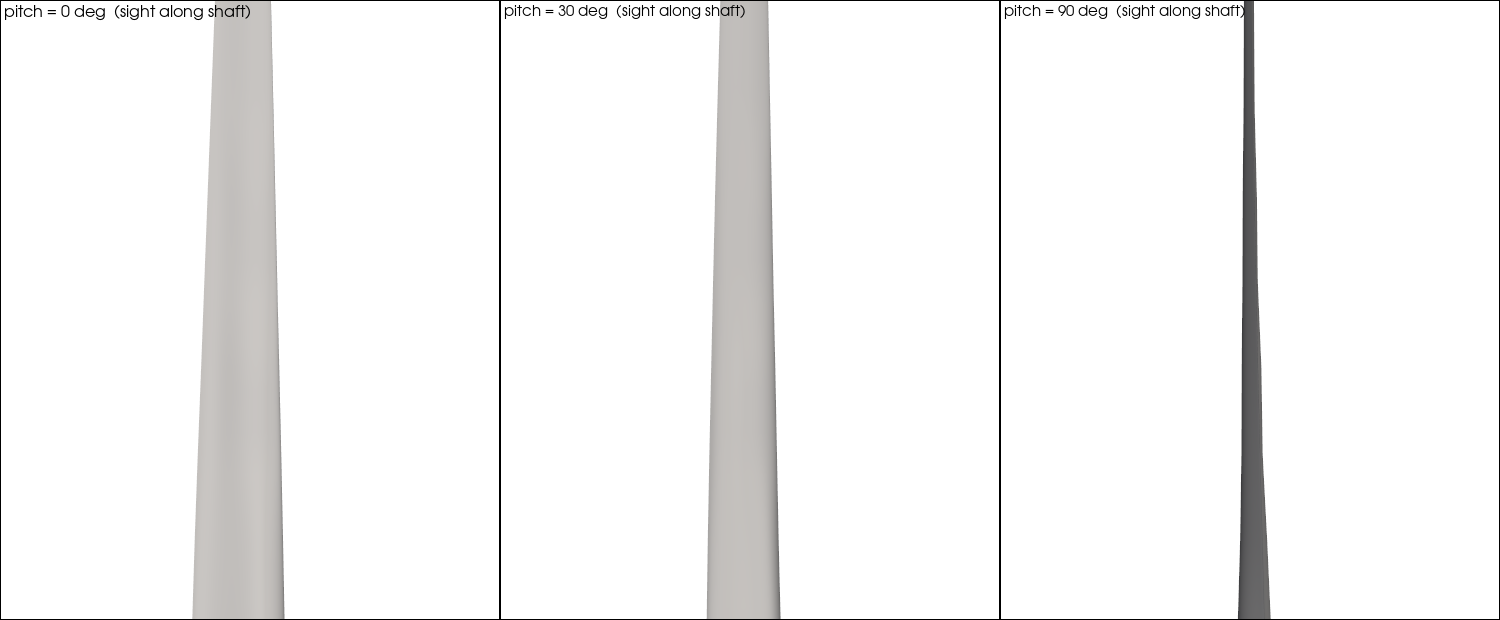
\includegraphics[width=\linewidth]{figs/fig_blade_pitch.png}\\
      {\scriptsize 叶片真实几何与姿态（pitch / 自转 / 柔性变形）}
    \end{column}
  \end{columns}
\end{frame}

% =====================================================================
\section{当前实现与下一步}

\begin{frame}{当前实现（一）：物理仿真应用}
  \begin{columns}[T]
    \begin{column}{0.54\textwidth}
      \begin{itemize}\small
        \item \hl{场景即事实来源}：一份场景文件（YAML）决定机位、机型、来流、
              传感器——改文件，仿真与 3D 画面\textbf{一起变}；
        \item \hl{交互式 3D 视图}：地形、\term{wake}{尾流}热力图、机组姿态、
              传感器可视化；数据通道可\textbf{订阅/取消}（取消即真正停止采样）；
        \item 应用外壳（Studio）：场景 / 数据通道 / 训练 / 物理约束四面板围绕
              一个 3D 视图，训练在\textbf{后台线程}、界面响应流畅。
      \end{itemize}
    \end{column}
    \begin{column}{0.46\textwidth}
      \centering
      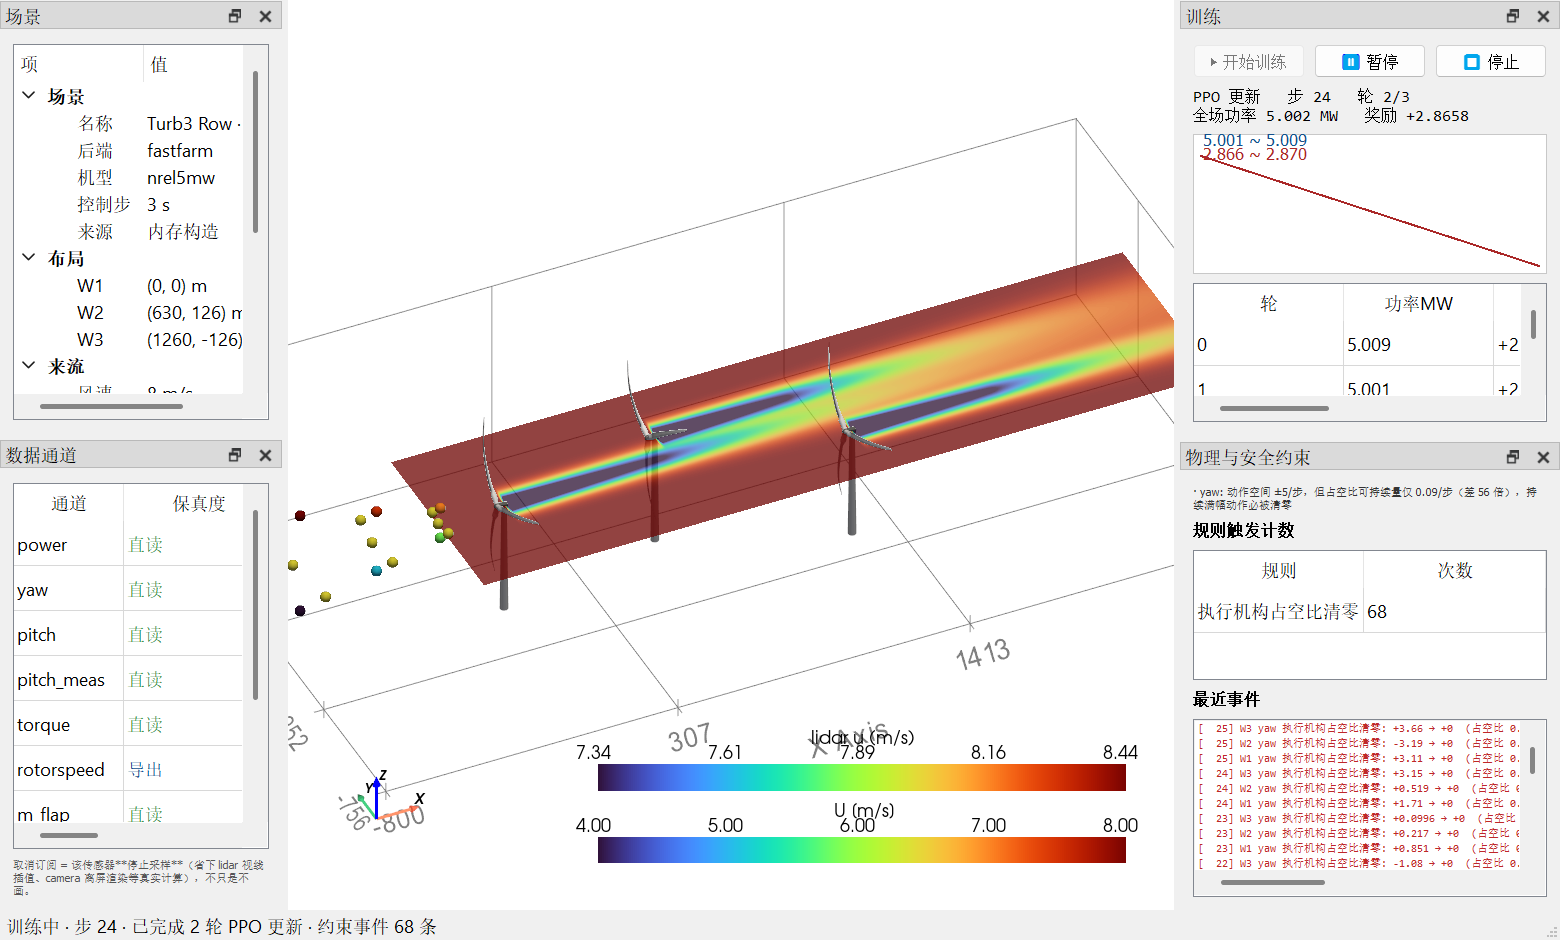
\includegraphics[width=\linewidth]{figs/fig_studio_overview.png}\\
      {\scriptsize Studio 应用外壳：3D 视图 $+$ 四面板}
    \end{column}
  \end{columns}
\end{frame}

\begin{frame}{当前实现（二）：RL 控制 $+$ 物理安全约束}
  \begin{itemize}\small
    \item \hl{多智能体强化学习}控制风电场协同：控制量为\term{yaw / pitch / torque}
          {偏航 / 变桨 / 转矩}，均经物理与安全约束层核验后下发；
    \item 训练\textbf{在平台内后台运行}，功率/奖励曲线、被改写动作的事件实时可见；
    \item 策略可\hl{保存并回放}到 3D，观测其实时控制；
    \item 稳定性由\hlr{约束层}保证——无论策略训练到什么程度，下发动作恒合物理。
  \end{itemize}
  \vfill
  \begin{center}
    \begin{tikzpicture}[font=\scriptsize]
      \node[draw,rounded corners,fill=mygreen!12] (a) {物理仿真应用 \checkmark};
      \node[draw,rounded corners,fill=mygreen!12,right=0.4cm of a] (b)
        {RL 控制 $+$ safety \checkmark};
      \node[draw,rounded corners,fill=mygreen!12,right=0.4cm of b] (c)
        {多模态传感通道 \checkmark};
      \node[draw,rounded corners,fill=mygreen!12,right=0.4cm of c] (d)
        {离线功能 / 可复现 \checkmark};
    \end{tikzpicture}
  \end{center}
\end{frame}

\begin{frame}{当前实现（三）：离线功能与受控实验}
  \begin{itemize}\small
    \item \hl{离线场景与几何工具}：不启动重仿真也能摆机组姿态、切地形、看相机视野
          与传感器布置——快速迭代方案；
    \item \hl{双物理后端}：稳态解析（FLORIS，秒级，适合大规模训练）与气动弹性
          （FAST.Farm，高保真，适合最终验证）\textbf{共用同一套管线}，可作受控对照；
    \item \hl{受控实验方法学}：来流可钉死、结论都有对照支撑、不可信数字会撤回；
    \item 每一路数据标注保真度与来源，汇报时可追溯。
  \end{itemize}
\end{frame}

\begin{frame}{当前实现（四）：约束\emph{入回路}后的一次真训练}
  \begin{center}\small
    把执行机构约束从“事后记录”真正\hl{接进学习回路}，跑满 40 轮真 FAST.Farm 训练。
    \textbf{加了什么、怎么加的}：
  \end{center}
  \vspace{-0.2em}
  \begin{columns}[T]
    \begin{column}{0.5\textwidth}
      \begin{block}{两处约束接进 obs 与 reward}
        \begin{itemize}\scriptsize
          \item \hl{占空比余量入观测}：obs 追加剩余占空比预算一列（$\text{维度}\,3\!\to\!4$）
                ——让策略\textbf{看得见}自己的动作会不会被整步清零；
          \item \hl{占空比惩罚入奖励}：动作被清零时按被吃掉的幅度给负奖励（$\lambda=0.5$）
                ——把“下发了却没执行”的空动作\textbf{记成代价}；
          \item 占空比口径改\hl{滑动窗口}（尾随 10 步累计上限 30\%），贴合执行机构的
                \textbf{预算}语义，而非逐步瞬时限幅。
        \end{itemize}
      \end{block}
      \begin{center}\scriptsize\color{mygray}
        这不是“让策略更强”的技巧——约束一直都在，区别只是策略\emph{此前看不见}它、
        于是学到一串\emph{从未被执行}的动作。
      \end{center}
    \end{column}
    \begin{column}{0.5\textwidth}
      \centering
      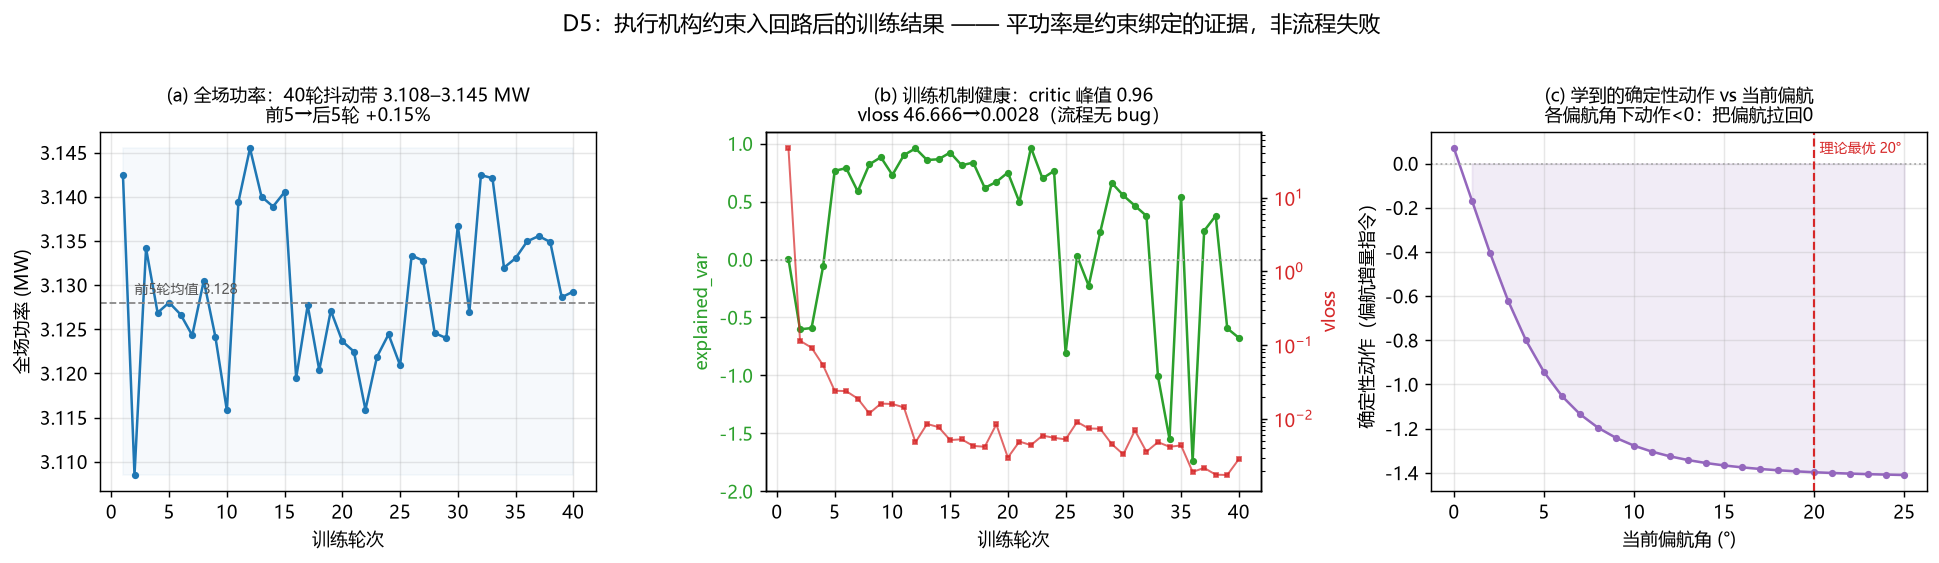
\includegraphics[width=\linewidth]{figs/fig_d5_binding.png}\\[0.3em]
      \begin{block}{读到了什么（\hlr{平功率本身就是结论}）}
        \begin{itemize}\scriptsize
          \item 功率全程 $3.11\!\sim\!3.15$\,MW 抖动、前5$\to$后5轮仅 $+0.15\%$，\textbf{无系统性增益}；
          \item 但 \term{critic}{价值网络} explained\_var 峰值 \hlg{0.96}、vloss 降 4 个量级
                $\Rightarrow$ 训练流程\textbf{健康}，非 bug；
          \item 学到的策略把偏航压回 $0$（均值 $0.93^\circ$），\textbf{够不到最优 $20^\circ$}——
                $0.09^\circ$/步 $\times\,170$ 步 $\approx 15^\circ$ 上限，\hlr{最优在回合内物理不可达}。
        \end{itemize}
      \end{block}
    \end{column}
  \end{columns}
\end{frame}

\begin{frame}{下一步：面向风场专业人员的内部试用版}
  \begin{columns}[T]
    \begin{column}{0.5\textwidth}
      \textbf{易用性（专业人员可上手）}
      \begin{itemize}\small
        \item \hl{可视化建场}：拖拽摆机组、导入数据通道，无需写配置；
        \item 场景/传感器/相机方案的\textbf{预设库}与一键对照；
        \item 更丰富的流场呈现（多切面、等值面 isosurface）。
      \end{itemize}
      \vspace{0.3em}
      \textbf{物理与控制的深化}
      \begin{itemize}\small
        \item \hl{解开约束绑定}：约束已入回路，但当前回合长度$\times$偏航速率上限让
              最优偏航物理不可达——加长回合 / 放大动作缩放 / 换 reference 奖励；
        \item \hl{疲劳载荷（DEL）纳入奖励}，做 power–fatigue 权衡；
        \item 变风况训练，得到\textbf{大小风况通用}的策略。
      \end{itemize}
    \end{column}
    \begin{column}{0.5\textwidth}
      \textbf{迈向愿景（远期）}
      \begin{itemize}\small
        \item \hl{多模态 $+$ 视觉语言模型（VLM）}：以 camera/vibration/acoustic
              为输入的感知–决策一体策略；
        \item \hl{市场化调度}：结合电力市场需求与实时风况，优化全场调度；
        \item 从 3 机组扩展到\textbf{真实规模风场}。
      \end{itemize}
      \vspace{0.3em}
      \begin{block}{Milestone}
        \small 下一版目标：\hlg{可供风场专业人员内部试用}——
        创建风场、导入数据、预演工业方案、在 3D 中观测全程。
      \end{block}
    \end{column}
  \end{columns}
\end{frame}

\begin{frame}{路线图总览}
  \small
  \begin{tabular}{@{}p{0.30\textwidth} p{0.40\textwidth} c@{}}
    \toprule
    \textbf{模块} & \textbf{内容} & \textbf{状态}\\
    \midrule
    物理仿真应用 & 场景即事实、交互 3D、双后端 & \hlg{\checkmark}\\
    RL 控制 $+$ safety & MAPPO $+$ 物理安全约束层 & \hlg{\checkmark}\\
    多模态传感通道 & camera/lidar/vibration/acoustic & \hlg{\checkmark}\\
    离线功能 / 可复现 & 几何工具、受控实验方法学 & \hlg{\checkmark}\\
    约束进学习回路 & obs 加占空比余量 $+$ 清零入奖励，40 轮实测 & \hlg{\checkmark}\\
    解开约束绑定 & 加长回合 / 放大缩放，让最优偏航可达 & 进行中\\
    疲劳载荷入奖励 & rainflow$\to$S-N$\to$Miner$\to$DEL & 输入已有，待接入\\
    变风况通用策略 & 大小风况泛化 & 进行中\\
    多模态 VLM 策略 & 感知–决策一体 & 远期\\
    市场化调度 & 市场需求 $+$ 风况优化 & 远期\\
    \bottomrule
  \end{tabular}
\end{frame}

\begin{frame}{小结}
  \begin{itemize}\setlength\itemsep{0.5em}
    \item 我们在做\hl{面向风电场的高保真物理仿真平台}——让控制策略与工业应用在
          上机前先在虚拟风场预演；
    \item 迫切性来自\hl{政策、市场与运维}三重压力，以及智能运维/风机智驾对高保真
          仿真的依赖；
    \item 立身之本是\hlr{严格的物理}：aeroelastic 底层、真实几何、数据分保真度、
          控制过物理与安全约束——\textbf{可验证、可复现、可证伪}；
    \item \hl{强化学习}是“无标签、强耦合、长时延”问题的对口方法；\hl{疲劳载荷}
          的物理输入已具备、估计方法成熟，下一步纳入优化目标；
    \item 当前已实现物理仿真 $+$ RL 控制 $+$ 安全约束 $+$ 多模态感知 $+$ 离线功能；
          下一版面向\hl{风场专业人员内部试用}，并向多模态 VLM 与市场化演进。
  \end{itemize}
  \vfill
  \begin{center}
    \large \hl{物理保真的“预演场”——让风电场的每一次工程决策先在仿真里跑一遍。}
  \end{center}
\end{frame}

\end{document}
